%%%%% Don't Make Changes Below Here %%%%%
\documentclass{article}\usepackage[utf8]{inputenc}\usepackage[margin=0.4cm,top=0.4cm,bottom=0.4cm]{geometry}\usepackage[usenames,dvipsnames,svgnames,table]{xcolor}\usepackage{calligra}\usepackage{tikz}\usetikzlibrary{matrix,fit,chains,calc,scopes}\usepackage{tcolorbox}\tcbuselibrary{skins}\tcbset{Baystyle/.style={sharp corners,enhanced,boxrule=6pt,colframe=Green,height=\textheight,width=\textwidth,borderline={8pt}{-11pt}{},}}\usepackage{amsmath,amssymb,amsthm,tikz,tkz-graph,color,chngpage,soul,hyperref,csquotes,graphicx,floatrow}\newcommand*{\QEDB}{\hfill\ensuremath{\square}}\newtheorem*{prop}{Proposition}\renewcommand{\theenumi}{\alph{enumi}}\usepackage[shortlabels]{enumitem}\usetikzlibrary{matrix,calc}\MakeOuterQuote{"}\newtheorem{theorem}{Theorem} \usetikzlibrary{shapes} \usepackage{lipsum}\usepackage{tabularx,ragged2e,booktabs,caption}\tcbuselibrary{breakable}\newenvironment{yframed}{\begin{tcolorbox}[breakable,colback=gray!3,title after break={\textit{\color{red}Solution (cont.)}},colbacktitle=gray!3, coltitle=black,titlerule=-1pt] }{\end{tcolorbox}}\newtcolorbox{mybox}{colback=black!15!white, colframe=white,arc=12pt}\newtcolorbox{myboxot}{colback=green!15!white, colframe=white,arc=12pt}\newtcbox{\mylib}{enhanced,boxrule=0pt,top=0mm,bottom=0mm,right=0mm,left=4mm,arc=4pt,boxsep=9pt,before upper={\vphantom{dlg}},colframe=green!50!black,coltext=green!25!black,colback=green!10!white,overlay={\begin{tcbclipinterior}\fill[green!75!blue!50!white] (frame.south west)rectangle node[text=white,font=\sffamily\bfseries\tiny,rotate=90] {Problem} ([xshift=4mm]frame.north west);\end{tcbclipinterior}}}\newtcbox{\mylibot}{enhanced,boxrule=0pt,top=0mm,bottom=0mm,right=0mm,arc=4pt,boxsep=9pt,before upper={\vphantom{dlg}},colframe=green!50!black,coltext=green!25!black,colback=green!10!white,overlay={\begin{tcbclipinterior}\fill[red!75!blue!50!white] (frame.south west)rectangle node[text=white,font=\sffamily\bfseries\tiny,rotate=90] {Other} ([xshift=4mm]frame.north west);\end{tcbclipinterior}}}\usepackage{algorithm}\usepackage[noend]{algpseudocode}\makeatletter\def\BState{\State\hskip-\ALG@thistlm}\makeatother\def\T{\indent}\def\star{\bigstar}
\def\Title{\begin{tcolorbox}[Baystyle,]{\begin{center}\vspace*{0.14\textheight}
{\rule{\textwidth}{1.6pt}\vspace*{-\baselineskip}\vspace*{2pt}}

\rule{\textwidth}{0.4pt}\\[0.2\baselineskip]{\fontsize{45}{45}\scshape CS 170: Efficient Algorithms and \\[-0.3\baselineskip] Intractable Problems \\[0.2\baselineskip] \calligra Spring 2017 \\[0.2\baselineskip]}
{\rule{\textwidth}{0.4pt}\vspace*{-\baselineskip}\vspace{3.2pt}}

% change homework number here
\rule{\textwidth}{1.6pt}\\[\baselineskip]\vspace{0.05\textheight}{{\fontsize{45}{45}\scshape$\bullet$\\ {Homework 7}\\ 
% change due date here
\vspace*{0.01\textheight} }{{\fontsize{18}{18}\scshape{Due on April 4 at 12:00pm\\}}}\fontsize{45}{45}\scshape$\bullet$  \\}

\vspace*{0.1\textheight}{\fontsize{12}{12}\calligra Solutions by\\}{\fontsize{28}{28}\scshape \Name \\}\vspace*{0.01\textheight}{\fontsize{12}{12}\scshape \SID} \\\vspace*{0.05\textheight}{\fontsize{12}{12}\calligra In collaboration with\\}\vspace*{0.01\textheight}{\fontsize{12}{12}\scshape \Collabs} \\\vspace*{0.05\textheight}\end{center}}\end{tcolorbox}\newgeometry{margin=0.75in}}\def\BeginSolution{\begin{yframed}\textbf{\color{red}Solution }}\def\EndSolution{\end{yframed}}
%%%%% Don't Make Changes Above Here %%%%%
\usepackage{fancyvrb}
%%%%% Template Begins Here %%%%%

\def\Name{John Wick}  % Your name 
\def\SID{01234567}  % Your student ID number
\def\Collabs{Doggo, Baba Yaga} % Your collaborators here with a comma between each person's name. Write None if no collaborators. Don't leave blank.


\pagestyle{empty}
\begin{document}
\Title

%%%% Problem 1 Starts Here %%%%
\vspace{1mm}\noindent\begin{mybox}{\begin{center}\textbf{\color{black}
% change problem name here
Problem 1: Linear Programming Fundamentals
}\end{center}}\end{mybox}\vspace{1mm}
% change difficulty level here
\begin{myboxot}\noindent\textbf{$\star$ Level}\end{myboxot} 
\noindent For each of the following optimization problems, is there a finite optimal solution that can be found by an LP solver? If the answer is no, identify the reason why (i.e. unbounded, infeasible, or not a linear program).
\begin{enumerate}[(a)]
	\item \[\text{max }5x+3y\]\begin{align*}
		x^2+y\le&45\\
		x\le&7\\
		x,y\ge&0
	\end{align*}
\BeginSolution % 1a
% Solution Here

\EndSolution
	\item \[\text{max }8x + \frac{1}{13}y+z\]\begin{align*}
		x\le&5\\
		4x+3z\le&9\\
		x,y,z\ge&0
	\end{align*}
\BeginSolution % 1b
% Solution Here

\EndSolution
\pagebreak
	\item \[\text{max }3x+3y\]\begin{align*}
		5x-2y\ge&0\\
		2x\le&18\\
		x,y\ge&0
	\end{align*}
\BeginSolution % 1c
% Solution Here

\EndSolution
	\item \[\text{max }2x+2y\]\begin{align*}
		x+2y \le& 12\\
		x \le& 6\\
		x+y \ge& 10\\
		x,y \ge& 0
	\end{align*}
\BeginSolution % 1d
% Solution Here

\EndSolution
	\item \[\text{max }2x-3y\]\begin{align*}
		3x+5y \ge & 13\\
		x \le & 4\\
		x,y \ge & 0
	\end{align*}
\BeginSolution % 1e
% Solution Here

\EndSolution
\end{enumerate}

%%%% Problem 1 Ends Here %%%%
\clearpage

%%%% Problem 2 Starts Here %%%%
\vspace{1mm}\noindent\begin{mybox}{\begin{center}\textbf{\color{black}
% change problem name here
Problem 2: Matches for tutoring
}\end{center}}\end{mybox}\vspace{1mm}
% change difficulty level here
\begin{myboxot}\noindent\textbf{$\star\star\star$ Level}\end{myboxot} 

\noindent A tutoring service has contracted you to work on pairing tutors with tutees. You are given a set of tutors $U$ and a set of tutees $V$. Everyone has filled out some questionnaires, so you know which tutors are compatible with which tutees (i.e. able to tutor the right subject). Additionally, each tutor i has given a limit $c_i$ on how many tutees they want to work with. Each tutee only gets one tutor. Describe an efficient algorithm for assigning tutors to tutees, such that as many tutees receive tutoring as possible. Give only the main idea.

\vspace{5pt}
\BeginSolution

\EndSolution

%%%% Problem 2 Ends Here %%%%
\clearpage

%%%% Problem 3 Starts Here %%%%
\vspace{1mm}\noindent\begin{mybox}{\begin{center}\textbf{\color{black}
% change problem name here
Problem 3: Criminal capture
}\end{center}}\end{mybox}\vspace{1mm}
% change difficulty level here
\begin{myboxot}\noindent\textbf{$\star\star\star\star$ Level}\end{myboxot} 
\noindent The Central Intelligence Agency has tasked you with preventing a criminal from fleeing the country. Roads and cities are represented as an unweighted directed graph $G = (V,E)$. We’re also given a set $C \subseteq V$ of possible current locations of the criminal, and a set $P \subseteq V$ of all airports out of the country. You want to set up roadblocks on a subset of the roads to prevent the criminal from escaping (i.e. reaching an airport).

\vspace*{5pt}
\noindent Clearly you could just put a roadblock at all the roads to each airport, but there might be a better way: for example, if the criminal is known to be at a particular intersection, you could just block all roads coming out of it. You may assume that roadblocks can be set up instantaneously.

\vspace*{5pt}
\noindent Give an efficient algorithm to find a way to stop the criminal using the least number of roadblocks.
\begin{enumerate}[(a)]
	\item Describe the main idea of your algorithm (no proof or pseudocode necessary).
	\BeginSolution % 3a
	
	\EndSolution
	\item Analyze the asymptotic running time of your algorithm, in terms of $|C|, |P|, |V|, and |E|$.
	\BeginSolution % 3b
	
	\EndSolution
	\item Unfortunately we were too slow in implementing your roadblocks. The criminal has made it to an
	airport and is flying from city to city within the country. Your only option now is to shut down entire airports. Naturally, you want to minimize the number of airports you must shut down.
	
	\vspace*{5pt}
	We formulate this as a graph problem where $V$ is now the set of airports, and the (directed) edges $E$ represent flights from one airport to another. We still know a set $C \subseteq V$ of possible current locations of the criminal, and $P \subseteq V$ the set of all airports with flights leaving the country. Give an efficient algorithm to find the minimal set of airports (vertices) to block that will prevent the criminal from reaching $P$.
	\BeginSolution % 3c
	
	\EndSolution
\end{enumerate}

%%%% Problem 3 Ends Here %%%%
\clearpage

%%%% Problem 4 Starts Here %%%%
\vspace{1mm}\noindent\begin{mybox}{\begin{center}\textbf{\color{black}
% change problem name here
Problem 4: Another max flow algorithm
}\end{center}}\end{mybox}\vspace{1mm}
% change difficulty level here
\begin{myboxot}\noindent\textbf{$\star\star\star\star\star$ Level}\end{myboxot} 
\noindent Consider the following simple network with edge capacities as shown.

\begin{center}
	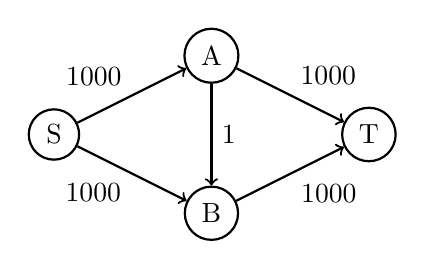
\begin{tikzpicture}[->,auto]
	\begin{scope}[every node/.style={circle,thick,draw}]
	\node (S) at (0,0) {S};
	\node (A) at (2,1) {A};
	\node (B) at (2,-1) {B};
	\node (T) at (4,0) {T};
	\end{scope}
	\begin{scope}[every edge/.style={draw,thick}]
	\path (S) edge node {$1000$} (A)
	          edge node[below,xshift=-14pt] {$1000$} (B)
		  (A) edge node {$1000$} (T)
		      edge node {$1$} (B)
		  (B) edge node[below,xshift=14pt] {$1000$} (T);
	
	\end{scope}
	\end{tikzpicture}
\end{center}

\begin{enumerate}[(a)]
\item Show that, if the Ford-Fulkerson algorithm is run on this graph, a careless choice of updates might cause it to take 2000 iterations. Imagine if the capacities were a million instead of 2000!
\BeginSolution

\EndSolution

\item We will now find a strategy for choosing paths under which the algorithm is guaranteed to terminate
in a reasonable number of iterations. 

\vspace{5pt}
Consider an arbitrary directed network $(G = (V,E), s, t,\{c_e\})$ in which we want to find the maximum flow. Assume for simplicity that all edge capacities are at least 1, and define the capacity of an $s-t$ path to be the smallest capacity of its constituent edges. The fattest path from $s$ to $t$ is the path with the most capacity.

\vspace{5pt}
Show how to modify Dijkstra’s algorithm to compute the fattest $s-t$ path in a graph. The full four-part algorithm response is not needed, but provide a convincing justification that your modification finds this path.
\BeginSolution

\EndSolution
\item Show that the maximum flow in $G$ is the sum of individual flows along at most $|E|$ paths from $s$ to $t$.
\BeginSolution

\EndSolution
\item Now show that if we always increase flow along the fattest path in the residual graph, then the Ford-Fulkerson algorithm will terminate in at most $O(|E| \log F)$ iterations, where $F$ is the size of the maximum flow. (Hint: It might help to recall the proof for the greedy set cover algorithm in Section
5.4.)

\vspace{5pt}
In fact, an even simpler rule—finding a path in the residual graph using breadth-first search—guarantees
that at most $O(|V| \cdot |E|)$ iterations will be needed.
\BeginSolution

\EndSolution
\end{enumerate}

%%%% Problem 4 Ends Here %%%%
\clearpage


%%%% Problem 5 Starts Here %%%%
\vspace{-2mm}\noindent\begin{mybox}{\begin{center}\textbf{\color{black}
% change problem name here
Problem 5: Cannibal canisters
}\end{center}}\end{mybox}
\begin{myboxot}\noindent\textbf{$\star\star\star\star\star$ Level}\end{myboxot} 

\noindent You see n canisters, each with their own height $h_i$ and radius $r_i$ (they are perfectly cylindrical). A canister can eat another canister if it has a smaller height and radius. The eaten canister will be instantly consumed, and the eating canister will be tired for the rest of the day, unable to eat anymore. Design an algorithm to make as many canisters as possible get eaten (so they don’t try to eat you!) by the end of the day. Your solution should give the optimal order that canisters should eat each other, and the runtime should be $O(n^3)$. 

\vspace{5pt}
\noindent As an example, if there are three canisters with height and radius:
\begin{gather*}
	h_1 = r_1 = 1.5\\
	h_2 = r_2 = 2.5\\
	h_3 = r_3 = 3.5
\end{gather*}Then your output should be "$c_2$ eats $c_1$, $c_3$ eats $c_2$" or similar.
\begin{enumerate}[(a)]
	\item For this part, assume that $\forall i,h_i = r_i$. How would you solve the problem? Describe only the main idea and runtime, no need for pseudocode or proof.
\BeginSolution

\EndSolution
	\item Solve the question fully, without the assumption that $h_i = r_i$. Hint: think about bipartite matching.
\BeginSolution

\EndSolution
\end{enumerate}

%%%% Problem 5 Ends Here %%%%

\end{document}
%%%%% Template Ends Here %%%%%
